\documentclass[
  stu,
  floatsintext,
  longtable,
  a4paper,
  nolmodern,
  notxfonts,
  notimes,
  donotrepeattitle,
  colorlinks=true,linkcolor=blue,citecolor=blue,urlcolor=blue]{apa7}

\usepackage{amsmath}
\usepackage{amssymb}

\usepackage[globalsuspend=true]{assoccnt}
\SuspendCounters{table}



\usepackage[bidi=default]{babel}
\babelprovide[main,import]{ngerman}


% get rid of language-specific shorthands (see #6817):
\let\LanguageShortHands\languageshorthands
\def\languageshorthands#1{}

\RequirePackage{longtable}
\RequirePackage{threeparttablex}

\makeatletter
\renewcommand{\paragraph}{\@startsection{paragraph}{4}{\parindent}%
	{0\baselineskip \@plus 0.2ex \@minus 0.2ex}%
	{-.5em}%
	{\normalfont\normalsize\bfseries\typesectitle}}

\renewcommand{\subparagraph}[1]{\@startsection{subparagraph}{5}{0.5em}%
	{0\baselineskip \@plus 0.2ex \@minus 0.2ex}%
	{-\z@\relax}%
	{\normalfont\normalsize\bfseries\itshape\hspace{\parindent}{#1}\textit{\addperi}}{\relax}}
\makeatother




\usepackage{longtable, booktabs, multirow, multicol, colortbl, hhline, caption, array, float, xpatch}
\setcounter{topnumber}{2}
\setcounter{bottomnumber}{2}
\setcounter{totalnumber}{4}
\renewcommand{\topfraction}{0.85}
\renewcommand{\bottomfraction}{0.85}
\renewcommand{\textfraction}{0.15}
\renewcommand{\floatpagefraction}{0.7}

\usepackage{tcolorbox}
\tcbuselibrary{listings,theorems, breakable, skins}
\usepackage{fontawesome5}

\definecolor{quarto-callout-color}{HTML}{909090}
\definecolor{quarto-callout-note-color}{HTML}{0758E5}
\definecolor{quarto-callout-important-color}{HTML}{CC1914}
\definecolor{quarto-callout-warning-color}{HTML}{EB9113}
\definecolor{quarto-callout-tip-color}{HTML}{00A047}
\definecolor{quarto-callout-caution-color}{HTML}{FC5300}
\definecolor{quarto-callout-color-frame}{HTML}{ACACAC}
\definecolor{quarto-callout-note-color-frame}{HTML}{4582EC}
\definecolor{quarto-callout-important-color-frame}{HTML}{D9534F}
\definecolor{quarto-callout-warning-color-frame}{HTML}{F0AD4E}
\definecolor{quarto-callout-tip-color-frame}{HTML}{02B875}
\definecolor{quarto-callout-caution-color-frame}{HTML}{FD7E14}

%\newlength\Oldarrayrulewidth
%\newlength\Oldtabcolsep


\usepackage{hyperref}



\usepackage{color}
\usepackage{fancyvrb}
\newcommand{\VerbBar}{|}
\newcommand{\VERB}{\Verb[commandchars=\\\{\}]}
\DefineVerbatimEnvironment{Highlighting}{Verbatim}{commandchars=\\\{\}}
% Add ',fontsize=\small' for more characters per line
\usepackage{framed}
\definecolor{shadecolor}{RGB}{241,243,245}
\newenvironment{Shaded}{\begin{snugshade}}{\end{snugshade}}
\newcommand{\AlertTok}[1]{\textcolor[rgb]{0.68,0.00,0.00}{#1}}
\newcommand{\AnnotationTok}[1]{\textcolor[rgb]{0.37,0.37,0.37}{#1}}
\newcommand{\AttributeTok}[1]{\textcolor[rgb]{0.40,0.45,0.13}{#1}}
\newcommand{\BaseNTok}[1]{\textcolor[rgb]{0.68,0.00,0.00}{#1}}
\newcommand{\BuiltInTok}[1]{\textcolor[rgb]{0.00,0.23,0.31}{#1}}
\newcommand{\CharTok}[1]{\textcolor[rgb]{0.13,0.47,0.30}{#1}}
\newcommand{\CommentTok}[1]{\textcolor[rgb]{0.37,0.37,0.37}{#1}}
\newcommand{\CommentVarTok}[1]{\textcolor[rgb]{0.37,0.37,0.37}{\textit{#1}}}
\newcommand{\ConstantTok}[1]{\textcolor[rgb]{0.56,0.35,0.01}{#1}}
\newcommand{\ControlFlowTok}[1]{\textcolor[rgb]{0.00,0.23,0.31}{#1}}
\newcommand{\DataTypeTok}[1]{\textcolor[rgb]{0.68,0.00,0.00}{#1}}
\newcommand{\DecValTok}[1]{\textcolor[rgb]{0.68,0.00,0.00}{#1}}
\newcommand{\DocumentationTok}[1]{\textcolor[rgb]{0.37,0.37,0.37}{\textit{#1}}}
\newcommand{\ErrorTok}[1]{\textcolor[rgb]{0.68,0.00,0.00}{#1}}
\newcommand{\ExtensionTok}[1]{\textcolor[rgb]{0.00,0.23,0.31}{#1}}
\newcommand{\FloatTok}[1]{\textcolor[rgb]{0.68,0.00,0.00}{#1}}
\newcommand{\FunctionTok}[1]{\textcolor[rgb]{0.28,0.35,0.67}{#1}}
\newcommand{\ImportTok}[1]{\textcolor[rgb]{0.00,0.46,0.62}{#1}}
\newcommand{\InformationTok}[1]{\textcolor[rgb]{0.37,0.37,0.37}{#1}}
\newcommand{\KeywordTok}[1]{\textcolor[rgb]{0.00,0.23,0.31}{#1}}
\newcommand{\NormalTok}[1]{\textcolor[rgb]{0.00,0.23,0.31}{#1}}
\newcommand{\OperatorTok}[1]{\textcolor[rgb]{0.37,0.37,0.37}{#1}}
\newcommand{\OtherTok}[1]{\textcolor[rgb]{0.00,0.23,0.31}{#1}}
\newcommand{\PreprocessorTok}[1]{\textcolor[rgb]{0.68,0.00,0.00}{#1}}
\newcommand{\RegionMarkerTok}[1]{\textcolor[rgb]{0.00,0.23,0.31}{#1}}
\newcommand{\SpecialCharTok}[1]{\textcolor[rgb]{0.37,0.37,0.37}{#1}}
\newcommand{\SpecialStringTok}[1]{\textcolor[rgb]{0.13,0.47,0.30}{#1}}
\newcommand{\StringTok}[1]{\textcolor[rgb]{0.13,0.47,0.30}{#1}}
\newcommand{\VariableTok}[1]{\textcolor[rgb]{0.07,0.07,0.07}{#1}}
\newcommand{\VerbatimStringTok}[1]{\textcolor[rgb]{0.13,0.47,0.30}{#1}}
\newcommand{\WarningTok}[1]{\textcolor[rgb]{0.37,0.37,0.37}{\textit{#1}}}

\providecommand{\tightlist}{%
  \setlength{\itemsep}{0pt}\setlength{\parskip}{0pt}}
\usepackage{longtable,booktabs,array}
\usepackage{calc} % for calculating minipage widths
% Correct order of tables after \paragraph or \subparagraph
\usepackage{etoolbox}
\makeatletter
\patchcmd\longtable{\par}{\if@noskipsec\mbox{}\fi\par}{}{}
\makeatother
% Allow footnotes in longtable head/foot
\IfFileExists{footnotehyper.sty}{\usepackage{footnotehyper}}{\usepackage{footnote}}
\makesavenoteenv{longtable}

\usepackage{graphicx}
\makeatletter
\def\maxwidth{\ifdim\Gin@nat@width>\linewidth\linewidth\else\Gin@nat@width\fi}
\def\maxheight{\ifdim\Gin@nat@height>\textheight\textheight\else\Gin@nat@height\fi}
\makeatother
% Scale images if necessary, so that they will not overflow the page
% margins by default, and it is still possible to overwrite the defaults
% using explicit options in \includegraphics[width, height, ...]{}
\setkeys{Gin}{width=\maxwidth,height=\maxheight,keepaspectratio}
% Set default figure placement to htbp
\makeatletter
\def\fps@figure{htbp}
\makeatother


% definitions for citeproc citations
\NewDocumentCommand\citeproctext{}{}
\NewDocumentCommand\citeproc{mm}{%
  \begingroup\def\citeproctext{#2}\cite{#1}\endgroup}
\makeatletter
 % allow citations to break across lines
 \let\@cite@ofmt\@firstofone
 % avoid brackets around text for \cite:
 \def\@biblabel#1{}
 \def\@cite#1#2{{#1\if@tempswa , #2\fi}}
\makeatother
\newlength{\cslhangindent}
\setlength{\cslhangindent}{1.5em}
\newlength{\csllabelwidth}
\setlength{\csllabelwidth}{3em}
\newenvironment{CSLReferences}[2] % #1 hanging-indent, #2 entry-spacing
 {\begin{list}{}{%
  \setlength{\itemindent}{0pt}
  \setlength{\leftmargin}{0pt}
  \setlength{\parsep}{0pt}
  % turn on hanging indent if param 1 is 1
  \ifodd #1
   \setlength{\leftmargin}{\cslhangindent}
   \setlength{\itemindent}{-1\cslhangindent}
  \fi
  % set entry spacing
  \setlength{\itemsep}{#2\baselineskip}}}
 {\end{list}}
\usepackage{calc}
\newcommand{\CSLBlock}[1]{\hfill\break\parbox[t]{\linewidth}{\strut\ignorespaces#1\strut}}
\newcommand{\CSLLeftMargin}[1]{\parbox[t]{\csllabelwidth}{\strut#1\strut}}
\newcommand{\CSLRightInline}[1]{\parbox[t]{\linewidth - \csllabelwidth}{\strut#1\strut}}
\newcommand{\CSLIndent}[1]{\hspace{\cslhangindent}#1}



\setlength\parindent{1cm}
\setlength\parskip{0cm}




\usepackage{newtx}

\defaultfontfeatures{Scale=MatchLowercase}
\defaultfontfeatures[\rmfamily]{Ligatures=TeX,Scale=1}





\title{Beispielhafte Verwendung der Quarto Vorlage: Roadshow:}


\shorttitle{Quarto Vorlage}


\usepackage{etoolbox}






\author{Prof.~Dr.~Stephan huber}



\affiliation{
{Köln, NRW }}




\leftheader{huber}






\authornote{ 

\par{       }
\par{Correspondence concerning this article should be addressed to }
}

\makeatletter
\let\endoldlt\endlongtable
\def\endlongtable{
\hline
\endoldlt
}
\makeatother

\urlstyle{same}



\usepackage{booktabs}
\usepackage{longtable}
\usepackage{array}
\usepackage{multirow}
\usepackage{wrapfig}
\usepackage{float}
\usepackage{colortbl}
\usepackage{pdflscape}
\usepackage{tabu}
\usepackage{threeparttable}
\usepackage{threeparttablex}
\usepackage[normalem]{ulem}
\usepackage{makecell}
\usepackage{xcolor}
\usepackage{fontspec}
\usepackage{multicol}
\usepackage{hhline}
\newlength\Oldarrayrulewidth
\newlength\Oldtabcolsep
\usepackage{hyperref}
\makeatletter
\@ifpackageloaded{caption}{}{\usepackage{caption}}
\AtBeginDocument{%
\ifdefined\contentsname
  \renewcommand*\contentsname{Inhaltsverzeichnis}
\else
  \newcommand\contentsname{Inhaltsverzeichnis}
\fi
\ifdefined\listfigurename
  \renewcommand*\listfigurename{Abbildungsverzeichnis}
\else
  \newcommand\listfigurename{Abbildungsverzeichnis}
\fi
\ifdefined\listtablename
  \renewcommand*\listtablename{Tabellenverzeichnis}
\else
  \newcommand\listtablename{Tabellenverzeichnis}
\fi
\ifdefined\figurename
  \renewcommand*\figurename{Abbildung}
\else
  \newcommand\figurename{Abbildung}
\fi
\ifdefined\tablename
  \renewcommand*\tablename{Tabelle}
\else
  \newcommand\tablename{Tabelle}
\fi
}
\@ifpackageloaded{float}{}{\usepackage{float}}
\floatstyle{ruled}
\@ifundefined{c@chapter}{\newfloat{codelisting}{h}{lop}}{\newfloat{codelisting}{h}{lop}[chapter]}
\floatname{codelisting}{Listing}
\newcommand*\listoflistings{\listof{codelisting}{Listingverzeichnis}}
\makeatother
\makeatletter
\makeatother
\makeatletter
\@ifpackageloaded{caption}{}{\usepackage{caption}}
\@ifpackageloaded{subcaption}{}{\usepackage{subcaption}}
\makeatother

% From https://tex.stackexchange.com/a/645996/211326
%%% apa7 doesn't want to add appendix section titles in the toc
%%% let's make it do it
\makeatletter
\xpatchcmd{\appendix}
  {\par}
  {\addcontentsline{toc}{section}{\@currentlabelname}\par}
  {}{}
\makeatother

\begin{document}

    \cleardoublepage
\thispagestyle{empty}
\hfill 
\includegraphics[width=20cm]{logo.png}\\
{\centering
  {\large Charlotte Fresenius Hochschule\\
Studiengang: Psychologie (B. Sc.)\\
 Studienort: Köln  \par
}
  \hbox{}\vskip 0cm plus 1fill
  {\Large \bfseries Roadshow: \par}
      \vspace{3ex}
  {\Large \bfseries Beispielhafte Verwendung der Quarto
Vorlage \\  \par}
      \vfill
      {\large Prof.~Dr.~Stephan huber \par}
      \vspace{0ex}
  { \par}
  \vspace{0ex}
    {\large  \par}
  \vspace{0ex}
  { \par}
    \vspace{0ex}
    {\large  \par}
  \vspace{0ex}
  { \par}
  \vspace{12ex}
  {\large Gutachter:  \par}
  \vfill
  {\bfseries\large Abgabedatum:  \par}
  \vspace{2ex}
  %
  \clearpage
}




\setcounter{secnumdepth}{5}

\setlength\LTleft{0pt}


\section*{Zusammenfassung}\label{zusammenfassung}
\addcontentsline{toc}{section}{Zusammenfassung}

\noindent  Diese Vorlage wurde von Prof.~Dr.~Stephan Huber angefertigt.
Sie baut auf Quarto extension \texttt{apaquarto} auf
(\citeproc{ref-Schneider2024quarto}{Schneider, 2024}).

\newpage
\thispagestyle{empty}
\tableofcontents

\newpage

\section{Einführung}\label{einfuxfchrung}

Dies ist eine Vorlage. Sie können sie verwenden, um Ihre studentische
Arbeit mit Quarto zu schreiben. Die Formatierung folgt den Richtlinien,
die in American Psychological Association
(\citeproc{ref-ConciseGuideAPA2020}{2020}) festgelegt wurden. Diese
Vorlage wurde von mir, Prof.~Dr.~Stephan Huber\footnote{Email:
  \texttt{stephan.huber@hs-fresenius.de}}, verfasst. Es sei erwähnt,
dass ich die Quarto Extension \texttt{apaquarto} von Schneider
(\citeproc{ref-Schneider2024quarto}{2024}) so angepasst habe, dass die
Vorlage den Anforderungen der Charlotte Fresenius Universität
entsprechen. Insbesondere die Titelseite wurde den Vorgaben entsprechend
erstellt. Falls Sie Verbesserungsvorschläge haben, lassen Sie es mich
bitte wissen. Wenn Sie Hilfe bei Quarto benötigen, können Sie gerne
während meiner Sprechstunde vorbeikommen.

Sie können die Vorlage mit den entsprechenden Dateien auf studynet und
hier: \url{https://github.com/hubchev/ewa_template} herunterladen.

In den folgenden Abschnitten zeige ich Ihnen ein wenig, wie Sie Quarto
verwenden, um Text zu schreiben und zu formatieren. Wenn Sie weitere
Informationen zu Quarto benötigen, können Sie bei Schneider
(\citeproc{ref-Schneider2024quarto}{2024}) und der Website
\url{https://quarto.org/} eine Menge Informationen erhalten.

\section{Kapitel}\label{kapitel}

Die Formatierung der Überschriften regelt APA strikt, siehe:
\url{https://apastyle.apa.org/style-grammar-guidelines/paper-format/headings}

\subsection{Dies ist ein Abschnitt}\label{dies-ist-ein-abschnitt}

Dies ist Text.

\subsubsection{Dies ist eine
Unterabschnitt}\label{dies-ist-eine-unterabschnitt}

Dies ist Text.

\section{Bilder}\label{bilder}

\subsection{Bilddateien einbinden}\label{sec-bildladen}

In Abbildung~\ref{fig-logo} sehen Sie das Logo der Universität. In
Abbildung~\ref{fig-logo2} wird das Logo kleiner dargestellt und mit
einer anderen Methode eingebunden. Beide Methoden sind jedoch praktisch
equivalent. Letzlich bietet das winzige Logo in
Abbildung~\ref{fig-logo3} eine weitere Methode, Bilder einzubinden.

\begin{figure}[t]

{\caption{{Ein großes Logo.}{\label{fig-logo}}}}


\includegraphics[width=3in,height=\textheight]{logo.png}

{\noindent \emph{Anmerkung.} Hier steht eine Notiz zum Bild.}

\end{figure}

\begin{figure}[t]

\caption{\label{fig-logo2}Ein mittelgroßes Logo.}


\includegraphics[width=0.3\textwidth,height=\textheight]{logo.png}

\emph{Anmerkung.} Hier steht auch eine Notiz zum Bild.

\end{figure}%

\begin{figure}[t]

{\caption{{Das winzige Logo der Universität.}{\label{fig-logo3}}}}


\includegraphics[width=1.07in,height=\textheight]{logo.png}

{\noindent \emph{Anmerkung.} Hier steht auch eine Notiz zum Bild.}

\end{figure}

\subsection{Mit R erzeugte Grafiken
einbinden}\label{mit-r-erzeugte-grafiken-einbinden}

In Abbildung~\ref{fig-plotcar} wird ein Scatterplot veranschaulicht
welcher direkt in R erzeugt wurde. Das hat den Vorteil, dass die
Datenerzeugung und Veranschaulichung direkt in Quarto geschieht. Die
Daten sind also immer aktuell, Änderungen können direkt hier vorgenommen
werden, die Arbeit ist komplett transparent und replizierbar. Darüber
hinaus erspart man sich das Abspeichern und Exportieren der Grafik.

\begin{figure}[t]

{\caption{{Das ist eine Überschrift für eine hässliche
Abbildung.}{\label{fig-plotcar}}}}

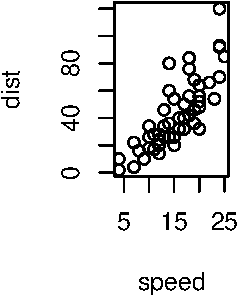
\includegraphics{roadshow_apa_de_files/figure-pdf/fig-plotcar-1.pdf}

{\noindent \emph{Anmerkung.} Hier steht auch eine Notiz zum Bild.}

\end{figure}

\section{Literatur einarbeiten}\label{literatur-einarbeiten}

\subsection{BibTeX}\label{bibtex}

Diese Vorlage kommt mit der Datei \texttt{literatur.bib}. Dies ist eine
BibTeX-Datei und erleichtert das Zitieren von Quellen und die Erstellung
von Literaturverzeichnissen. Hier ist eine Erklärung, wie eine
BibTeX-Datei funktioniert und warum sie nützlich ist.

Eine BibTeX-Datei ermöglicht es, alle Literaturangaben an einem Ort zu
speichern und zu organisieren. Dies erleichtert das Management der
Quellen, besonders bei umfangreichen Arbeiten. Quarto kann automatisch
auf die BibTeX-Datei zugreifen, um Zitate und Literaturverzeichnisse zu
erstellen. Dies spart Zeit und reduziert Fehler im Vergleich zum
manuellen Erstellen von Literaturverzeichnissen. Durch die Verwendung
einer BibTeX-Datei werden Zitate und Literaturverzeichnisse konsistent
formatiert, entsprechend den Vorgaben des jeweiligen Zitierstils. Ich
empfehle die Verwendung eines Literaturverwaltungsprogramms. Näheres
hierzu finden Sie in Kapitel~\ref{sec-jabref}.

Eine BibTeX-Datei ist eine textbasierte Datei mit der Erweiterung
\texttt{.bib}, die bibliografische Einträge enthält. Jeder Eintrag in
der Datei beschreibt eine Quelle (z. B. ein Buch, einen Artikel, eine
Website) und enthält verschiedene Felder wie Autor, Titel, Jahr und
Verlag. Ich habe beispielhaft alle möglichen teilweise fiktiven Einträge
in die Datei gepackt. Hier die ersten Zeilen der Datei:

\begin{Shaded}
\begin{Highlighting}[]
\NormalTok{@Article\{Huber2016,}
\NormalTok{  author    = \{Stephan Huber and Christoph Rust\},}
\NormalTok{  title     = \{osrmtime: Calculate Travel Time and Distance with \{OpenStreetMap\} Data Using the \{Open Source Routing Machine\} (\{OSRM\})\},}
\NormalTok{  journal   = \{The Stata Journal\},}
\NormalTok{  year      = \{2016\},}
\NormalTok{  volume    = \{16\},}
\NormalTok{  number    = \{2\},}
\NormalTok{  pages     = \{416{-}423\}}
\NormalTok{\}}
\end{Highlighting}
\end{Shaded}

Jeder Literatureintrag ist ähnlich strukturiert. Zuerst kommt die
Angabe, um welche Art der Literatur es sich handelt (hier:
\texttt{@Article}). Dann der sogenannte BibTeX-Key (hier:
\texttt{Huber2016}). Dieser ermöglicht es einen entsprechenden Verweis
im Text zu setzen, siehe Kapitel~\ref{sec-cite}. Zuletzt kommen die
Angaben, welche von dem gewählten Zitierstil (voreingestellt: APA 7)
weiter verarbeitet werden.

\subsection{Literaturverwaltung}\label{sec-jabref}

Eine BibTeX-Datei kann schnell unübersichtlich werden. Ich empfehle
daher die Verwendung eines Literaturverwaltungsprogramms wie JabRef,
siehe: \url{www.jabref.org}. Das Programm ist kostenlos und funktioniert
auf allen Ihren Geräten und mit allen Betriebssystemen. Insbesondere
kann es BibTeX-Dateien gut handhaben. Sie fragen sich vielleicht, was
eine BibTeX-Datei ist. Installieren Sie JabRef und öffnen Sie die Datei
\texttt{bibliography.bib} dieser Vorlage, dann werden Sie verstehen, was
ich meine.

\subsection{APA und CSL}\label{sec-apa}

Der vordefinierte Bibliographiestil dieser Vorlage ist APA in der 7.
Auflage. Sie können dies ändern. Hierzu einfach im (YAML) Header dieser
Vorlage den den entpsrechenden Stil angeben. Dies geschieht durch eine
Datei mit der Endung \texttt{csl} was für ``Citation Style Language''
steht. In dieser Datei sind die Zitierregeln ausgeführt so dass sie der
Computer umsetzen kann. Auf \url{https://www.zotero.org/styles} finden
Sie eine Vielzahl an Stilen. Wenn Sie beispielsweise APA in der 6.
Auflage verwenden wollen, gebe sie im Header folgendes an:

\begin{Shaded}
\begin{Highlighting}[]
\NormalTok{csl: "https://www.zotero.org/styles/apa{-}6th{-}edition"}
\end{Highlighting}
\end{Shaded}

\subsection{Literatur zitieren}\label{sec-cite}

In wissenschaftlichen Texten werden oft andere Arbeiten zitiert. Dies
kann auf unterschiedlichste Weise geschehen. Tabelle~\ref{tbl-letters}
zeigt, wie zitiert werden kann.

\begin{table}

{\caption{{So kann Literatur zitiert werden}{\label{tbl-letters}}}}

\begin{longtable}[]{@{}
  >{\raggedright\arraybackslash}p{(\columnwidth - 2\tabcolsep) * \real{0.4545}}
  >{\raggedright\arraybackslash}p{(\columnwidth - 2\tabcolsep) * \real{0.5455}}@{}}
\toprule\noalign{}
\begin{minipage}[b]{\linewidth}\raggedright
Code
\end{minipage} & \begin{minipage}[b]{\linewidth}\raggedright
So erscheint es im Text
\end{minipage} \\
\midrule\noalign{}
\endhead
\bottomrule\noalign{}
\endlastfoot
\texttt{@Huber2016} & Huber and Rust (\citeproc{ref-Huber2016}{2016}) \\
\texttt{@Huber2016{[}2{]}} & Huber and Rust
(\citeproc{ref-Huber2016}{2016, S. 2}) \\
\texttt{{[}@Huber2016{]}} & (\citeproc{ref-Huber2016}{Huber \& Rust,
2016}) \\
\texttt{{[}@Huber2016,\ 3-5{]}} & (\citeproc{ref-Huber2016}{Huber \&
Rust, 2016, S. 3--5}) \\
\texttt{{[}@Huber2016;\ @Aust2023{]}} & (\citeproc{ref-Aust2023}{Aust \&
Barth, 2023}; \citeproc{ref-Huber2016}{Huber \& Rust, 2016}) \\
\texttt{{[}Vgl.\ @Aust2023,\ S.\ 31;\ @Huber2016,\ S.\ 13{]}} & (Vgl.
\citeproc{ref-Aust2023}{Aust \& Barth, 2023, S. 31};
\citeproc{ref-Aust2023}{2023, S. 13}) \\
\end{longtable}

\end{table}

Hyperlinks kann man auch setzen: \texttt{{[}Google{]}(www.google.de)}
wird zu: \href{www.google.de}{Google}. Bei akademischen Arbeiten sollten
Quellen immer in das Literaturverzeichnis und Hyperlinks funktionieren
nicht in gedruckter Form. Hier ein Beispiel:
\href{www.google.de}{Google} ist eine beliebte Online-Suchmaschine
(siehe \citeproc{ref-Google2023Google}{Google, 2023}).

\subsection{Verschiedene Formate}

Hier sind einige fiktive Beispiele für verschiedene Arten von Literatur:
Unpublished (\citeproc{ref-unpublished}{1993}), WorkingPaper and
Arbeitspapier (\citeproc{ref-techreport}{1993}), PHD
(\citeproc{ref-phdthesis}{2011}), Misc (\citeproc{ref-misc}{1993}),
Masterthesis (\citeproc{ref-mastersthesis}{2004}), Editor
(\citeproc{ref-incollection}{2022}), Inbook
(\citeproc{ref-inbook}{1993}), Conference
(\citeproc{ref-conference}{1986}), Booklet
(\citeproc{ref-booklet}{1996}), Book (\citeproc{ref-book}{2023}),
Article (\citeproc{ref-article}{2011}), Proceedings
(\citeproc{ref-proceedings}{1993}), Website
(\citeproc{ref-webpage}{2023}).

Die entsprechende bibtex-Datei sollte die Einträge enthalten. Sie werden
angezeigt in Kapitel~\ref{sec-bibtexdatei}.

\section{Tabellen}\label{tabellen}

\subsection{Tabellen mit Markdown
erstellen}\label{tabellen-mit-markdown-erstellen}

Mit Markdown lassen sich Tabellen flexibel erstellen. Auf der Website
\url{https://quarto.org/docs/authoring/tables.html} werden die
Möglichkeiten erläutert. Tabelle~\ref{tbl-example} beispielsweise wird
mit Markdown Code erstellt.

\begin{table}

{\caption{{Eine beispielhafte Tabelle erstellt mit
Markdown}{\label{tbl-example}}}}

\begin{longtable}[]{@{}llrc@{}}
\toprule\noalign{}
Default & Left & Right & Center \\
\midrule\noalign{}
\endhead
\bottomrule\noalign{}
\endlastfoot
12 & 12 & 12 & 12 \\
123 & 123 & 123 & 123 \\
1 & 1 & 1 & 1 \\
\end{longtable}

{\noindent \emph{Anmerkung.} Hier ist eine Anmerkung.}

\end{table}

\subsection{Tabellen und Daten von R
einbinden}\label{tabellen-und-daten-von-r-einbinden}

Ein Beispiel, wie Objekte aus R in einer Tabelle dargestellt werden
können, findet sich in Tabelle~\ref{tbl-mixedtab}.

\begin{table}

{\caption{{Ein Tabelle mit deskriptiver
Statistik}{\label{tbl-mixedtab}}}}

\global\setlength{\Oldarrayrulewidth}{\arrayrulewidth}

\global\setlength{\Oldtabcolsep}{\tabcolsep}

\setlength{\tabcolsep}{2pt}

\renewcommand*{\arraystretch}{1.5}



\providecommand{\ascline}[3]{\noalign{\global\arrayrulewidth #1}\arrayrulecolor[HTML]{#2}\cline{#3}}

\begin{longtable*}[l]{|p{0.75in}|p{0.75in}|p{0.75in}|p{0.75in}|p{0.75in}|p{0.75in}}



\ascline{0.75pt}{000000}{1-6}

\multicolumn{1}{>{\centering}m{\dimexpr 0.75in+0\tabcolsep}}{\textcolor[HTML]{000000}{\fontsize{11}{22}\selectfont{\global\setmainfont{Times New Roman}{Dosage}}}} & \multicolumn{1}{>{\centering}m{\dimexpr 0.75in+0\tabcolsep}}{\textcolor[HTML]{000000}{\fontsize{11}{22}\selectfont{\global\setmainfont{Times New Roman}{Mean}}}} & \multicolumn{1}{>{\centering}m{\dimexpr 0.75in+0\tabcolsep}}{\textcolor[HTML]{000000}{\fontsize{11}{22}\selectfont{\global\setmainfont{Times New Roman}{Median}}}} & \multicolumn{1}{>{\centering}m{\dimexpr 0.75in+0\tabcolsep}}{\textcolor[HTML]{000000}{\fontsize{11}{22}\selectfont{\global\setmainfont{Times New Roman}{SD}}}} & \multicolumn{1}{>{\centering}m{\dimexpr 0.75in+0\tabcolsep}}{\textcolor[HTML]{000000}{\fontsize{11}{22}\selectfont{\global\setmainfont{Times New Roman}{Min}}}} & \multicolumn{1}{>{\centering}m{\dimexpr 0.75in+0\tabcolsep}}{\textcolor[HTML]{000000}{\fontsize{11}{22}\selectfont{\global\setmainfont{Times New Roman}{Max}}}} \\

\ascline{0.75pt}{000000}{1-6}\endfirsthead 

\ascline{0.75pt}{000000}{1-6}

\multicolumn{1}{>{\centering}m{\dimexpr 0.75in+0\tabcolsep}}{\textcolor[HTML]{000000}{\fontsize{11}{22}\selectfont{\global\setmainfont{Times New Roman}{Dosage}}}} & \multicolumn{1}{>{\centering}m{\dimexpr 0.75in+0\tabcolsep}}{\textcolor[HTML]{000000}{\fontsize{11}{22}\selectfont{\global\setmainfont{Times New Roman}{Mean}}}} & \multicolumn{1}{>{\centering}m{\dimexpr 0.75in+0\tabcolsep}}{\textcolor[HTML]{000000}{\fontsize{11}{22}\selectfont{\global\setmainfont{Times New Roman}{Median}}}} & \multicolumn{1}{>{\centering}m{\dimexpr 0.75in+0\tabcolsep}}{\textcolor[HTML]{000000}{\fontsize{11}{22}\selectfont{\global\setmainfont{Times New Roman}{SD}}}} & \multicolumn{1}{>{\centering}m{\dimexpr 0.75in+0\tabcolsep}}{\textcolor[HTML]{000000}{\fontsize{11}{22}\selectfont{\global\setmainfont{Times New Roman}{Min}}}} & \multicolumn{1}{>{\centering}m{\dimexpr 0.75in+0\tabcolsep}}{\textcolor[HTML]{000000}{\fontsize{11}{22}\selectfont{\global\setmainfont{Times New Roman}{Max}}}} \\

\ascline{0.75pt}{000000}{1-6}\endhead



\multicolumn{1}{>{\centering}m{\dimexpr 0.75in+0\tabcolsep}}{\textcolor[HTML]{000000}{\fontsize{11}{22}\selectfont{\global\setmainfont{Times New Roman}{A}}}} & \multicolumn{1}{>{\centering}m{\dimexpr 0.75in+0\tabcolsep}}{\textcolor[HTML]{000000}{\fontsize{11}{22}\selectfont{\global\setmainfont{Times New Roman}{14.19}}}} & \multicolumn{1}{>{\centering}m{\dimexpr 0.75in+0\tabcolsep}}{\textcolor[HTML]{000000}{\fontsize{11}{22}\selectfont{\global\setmainfont{Times New Roman}{14.00}}}} & \multicolumn{1}{>{\centering}m{\dimexpr 0.75in+0\tabcolsep}}{\textcolor[HTML]{000000}{\fontsize{11}{22}\selectfont{\global\setmainfont{Times New Roman}{4.45}}}} & \multicolumn{1}{>{\centering}m{\dimexpr 0.75in+0\tabcolsep}}{\textcolor[HTML]{000000}{\fontsize{11}{22}\selectfont{\global\setmainfont{Times New Roman}{5}}}} & \multicolumn{1}{>{\centering}m{\dimexpr 0.75in+0\tabcolsep}}{\textcolor[HTML]{000000}{\fontsize{11}{22}\selectfont{\global\setmainfont{Times New Roman}{25}}}} \\





\multicolumn{1}{>{\centering}m{\dimexpr 0.75in+0\tabcolsep}}{\textcolor[HTML]{000000}{\fontsize{11}{22}\selectfont{\global\setmainfont{Times New Roman}{B}}}} & \multicolumn{1}{>{\centering}m{\dimexpr 0.75in+0\tabcolsep}}{\textcolor[HTML]{000000}{\fontsize{11}{22}\selectfont{\global\setmainfont{Times New Roman}{13.50}}}} & \multicolumn{1}{>{\centering}m{\dimexpr 0.75in+0\tabcolsep}}{\textcolor[HTML]{000000}{\fontsize{11}{22}\selectfont{\global\setmainfont{Times New Roman}{14.00}}}} & \multicolumn{1}{>{\centering}m{\dimexpr 0.75in+0\tabcolsep}}{\textcolor[HTML]{000000}{\fontsize{11}{22}\selectfont{\global\setmainfont{Times New Roman}{5.15}}}} & \multicolumn{1}{>{\centering}m{\dimexpr 0.75in+0\tabcolsep}}{\textcolor[HTML]{000000}{\fontsize{11}{22}\selectfont{\global\setmainfont{Times New Roman}{4}}}} & \multicolumn{1}{>{\centering}m{\dimexpr 0.75in+0\tabcolsep}}{\textcolor[HTML]{000000}{\fontsize{11}{22}\selectfont{\global\setmainfont{Times New Roman}{22}}}} \\





\multicolumn{1}{>{\centering}m{\dimexpr 0.75in+0\tabcolsep}}{\textcolor[HTML]{000000}{\fontsize{11}{22}\selectfont{\global\setmainfont{Times New Roman}{C}}}} & \multicolumn{1}{>{\centering}m{\dimexpr 0.75in+0\tabcolsep}}{\textcolor[HTML]{000000}{\fontsize{11}{22}\selectfont{\global\setmainfont{Times New Roman}{19.19}}}} & \multicolumn{1}{>{\centering}m{\dimexpr 0.75in+0\tabcolsep}}{\textcolor[HTML]{000000}{\fontsize{11}{22}\selectfont{\global\setmainfont{Times New Roman}{19.00}}}} & \multicolumn{1}{>{\centering}m{\dimexpr 0.75in+0\tabcolsep}}{\textcolor[HTML]{000000}{\fontsize{11}{22}\selectfont{\global\setmainfont{Times New Roman}{3.52}}}} & \multicolumn{1}{>{\centering}m{\dimexpr 0.75in+0\tabcolsep}}{\textcolor[HTML]{000000}{\fontsize{11}{22}\selectfont{\global\setmainfont{Times New Roman}{13}}}} & \multicolumn{1}{>{\centering}m{\dimexpr 0.75in+0\tabcolsep}}{\textcolor[HTML]{000000}{\fontsize{11}{22}\selectfont{\global\setmainfont{Times New Roman}{25}}}} \\

\ascline{0.75pt}{000000}{1-6}



\end{longtable*}



\arrayrulecolor[HTML]{000000}

\global\setlength{\arrayrulewidth}{\Oldarrayrulewidth}

\global\setlength{\tabcolsep}{\Oldtabcolsep}

\renewcommand*{\arraystretch}{1}

{\noindent \emph{Anmerkung.} Eine Notiz.}

\end{table}

\subsection{Abschnitte setzen und Text
formatieren}\label{abschnitte-setzen-und-text-formatieren}

\subsubsection{Das ist Unterabschnitt}\label{das-ist-unterabschnitt}

Ein Abschnitt sollte nicht alleine kommen, daher\ldots{}

\subsubsection{Der zweite
Unterabschnitt}\label{der-zweite-unterabschnitt}

Hier gehört ihr Text.

\section{Text formatieren}\label{text-formatieren}

\textbf{This is bold text}

\textbf{This is bold text}

\emph{This is italic text}

\emph{This is italic text}

\subsection{Listen}\label{listen}

\begin{itemize}
\tightlist
\item
  Eine Liste erstellen, indem man eine Zeile mit \texttt{+}, \texttt{-}
  oder \texttt{*} beginnt
\item
  Unterlisten werden durch Einrücken um 2 Leerzeichen erstellt:

  \begin{itemize}
  \tightlist
  \item
    Ein Wechsel des Markierungszeichens erzwingt den Start einer neuen
    Liste:

    \begin{itemize}
    \tightlist
    \item
      bli
    \item
      bla
    \item
      blubb
    \end{itemize}
  \end{itemize}
\item
  Sehr einfach!
\end{itemize}

Nummerierte Listen sind einfach:

\begin{enumerate}
\def\labelenumi{\arabic{enumi}.}
\item
  Ein Argument.
\item
  Ein weiteres Argument.
\item
  Das beste Argument.
\item
  Man kann fortlaufende Zahlen verwenden\ldots{}
\item
  \ldots oder alle Zahlen als \texttt{1.} behalten
\end{enumerate}

Nummerierung mit einer höheren Zahl beginnen, geht auch:

\begin{enumerate}
\def\labelenumi{\arabic{enumi}.}
\setcounter{enumi}{56}
\tightlist
\item
  foo
\item
  bar
\end{enumerate}

\subsection{Code}\label{code}

R Objekte können direkt aufgerufen werden. Der Mittelwert der
Beobachtungen der Variable \emph{speed} die grafisch auf der x-Achse in
Abbildung~\ref{fig-plotcar} veranschaulicht sind ist 15.4.

\subsection{Formeln}\label{formeln}

Wenn \(a \ne 0\) ist, gibt es zwei Lösungen für die Gleichung
\((ax^2 + bx + c = 0)\) und sie lauten
\[ x = \frac{-b \pm \sqrt{b^2-4ac}}{2a} \]

\subsection{\texorpdfstring{\href{https://github.com/markdown-it/markdown-it-footnote}{Fußnoten}}{Fußnoten}}\label{fuuxdfnoten}

Fußnote 1 Verweis\footnote{Fußnote \textbf{kann Markup enthalten}

  und mehrere Absätze.}.

Fußnote 2 Verweis\footnote{Fußnotentext.}.

Inline Fußnote\footnote{Text der Inline-Fußnote} Definition.

Doppelter Fußnotenverweis\footnote{Fußnotentext.}.

\newpage

\section*{Literaturverzeichnis}\label{literaturverzeichnis}
\addcontentsline{toc}{section}{Literaturverzeichnis}

\phantomsection\label{refs}
\begin{CSLReferences}{1}{0}
\bibitem[\citeproctext]{ref-ConciseGuideAPA2020}
American Psychological Association. (2020). \emph{Concise Guide to {APA
Style}: {The} Official {APA Style} Guide for Students (7th Ed.).}
Author. \url{https://doi.org/10.1037/0000173-000}

\bibitem[\citeproctext]{ref-article}
Article, S. (2011). The title of the work. \emph{The name of the
journal}, \emph{4}(2), 201--213.

\bibitem[\citeproctext]{ref-Aust2023}
Aust, F., \& Barth, M. (2023). \emph{{papaja}: {Prepare} reproducible
{APA} journal articles with {R} Markdown}.
\url{https://github.com/crsh/papaja}

\bibitem[\citeproctext]{ref-book}
Book, D. (2023). \emph{The title of the work} (3. Aufl., Bd. 4). The
name of the publisher.

\bibitem[\citeproctext]{ref-booklet}
Booklet, B. (1996, Juli). \emph{The title of the work}. How it was
published.

\bibitem[\citeproctext]{ref-conference}
Conference, D. (1986). \emph{The title of the work} (T. editor, Hrsg.;
Bd. 4, S. 213). The organization; The publisher.

\bibitem[\citeproctext]{ref-incollection}
Editor, E. (2022). The title of the work. In T. editor (Hrsg.),
\emph{The title of the book} (3. Aufl., Bd. 4, S. 101--114). The name of
the publisher.

\bibitem[\citeproctext]{ref-Google2023Google}
Google. (2023). \emph{Google Search}. January 30, 2023.
\url{https://www.google.com/}

\bibitem[\citeproctext]{ref-Huber2016}
Huber, S., \& Rust, C. (2016). osrmtime: Calculate Travel Time and
Distance with {OpenStreetMap} Data Using the {Open Source Routing
Machine} ({OSRM}). \emph{The Stata Journal}, \emph{16}(2), 416--423.

\bibitem[\citeproctext]{ref-inbook}
Inbook, S. (1993). \emph{The title of the work} (3. Aufl., Bd. 4, S.
201--213). The name of the publisher.

\bibitem[\citeproctext]{ref-mastersthesis}
Masterthesis, A. (2004). \emph{The title of the work} {[}Mathesis{]}.
The school of the thesis.

\bibitem[\citeproctext]{ref-misc}
Misc, A. (1993). \emph{The title of the work}. How it was published.

\bibitem[\citeproctext]{ref-phdthesis}
PHD, A. (2011). \emph{The title of the work} {[}Phdthesis{]}. The school
of the thesis.

\bibitem[\citeproctext]{ref-proceedings}
Proceedings, L. (Hrsg.). (1993). \emph{The title of the work} (Bd. 4).
The organization; The name of the publisher.

\bibitem[\citeproctext]{ref-Schneider2024quarto}
Schneider, W. J. (2024). \emph{A quarto extension for creating APA7
documents in .docx, .html, and .pdf formats}.
\url{https://wjschne.github.io/apaquarto/}

\bibitem[\citeproctext]{ref-unpublished}
Unpublished, A. (1993). \emph{The title of the work}.

\bibitem[\citeproctext]{ref-webpage}
Website, A. (2023). \emph{Website Title}. \url{http://website-url.com}

\bibitem[\citeproctext]{ref-techreport}
WorkingPaper, P., \& Arbeitspapier, S. (1993). \emph{The title of the
work} (2). The institution that published.

\end{CSLReferences}

\newpage
\appendix

\section{Eine erster Anhang}\label{eine-erster-anhang}

Hier steht Text und Abbildung~\ref{fig-logo4}.

\begin{figure}[h]

{\caption{{Logo der CFH.}{\label{fig-logo4}}}}


\includegraphics[width=2in,height=\textheight]{logo.png}

{\noindent \emph{Anmerkung.} Das ist das Logo der CFH.}

\end{figure}

\newpage

\section{Eine zweiter Anhang}\label{eine-zweiter-anhang}

Hier steht Text und Abbildung~\ref{fig-logo5}.

\begin{figure}[h]

{\caption{{Schon wieder das Logo.}{\label{fig-logo5}}}}


\includegraphics[width=2in,height=\textheight]{logo.png}

{\noindent \emph{Anmerkung.} Das ist das Logo der CFH.}

\end{figure}

\newpage

\section{BibTex Datei}\label{sec-bibtexdatei}

\begin{Shaded}
\begin{Highlighting}[]
\NormalTok{    @Unpublished\{unpublished,}
\NormalTok{        author = \{Andy Unpublished\},}
\NormalTok{        title  = \{The title of the work\},}
\NormalTok{        month  = \{7\},}
\NormalTok{        year   = \{1993\},}
\NormalTok{    \}}
    
\NormalTok{    @TechReport\{techreport,}
\NormalTok{        author      = \{Peter WorkingPaper\},}
\NormalTok{        title       = \{The title of the work\},}
\NormalTok{        institution = \{The institution that published\},}
\NormalTok{        year        = \{1993\},}
\NormalTok{        number      = \{2\},}
\NormalTok{        address     = \{The address of the publisher\},}
\NormalTok{        month       = \{7\},}
\NormalTok{    \}}
    
\NormalTok{    @PhdThesis\{phdthesis,}
\NormalTok{        author  = \{Andreas PHD\},}
\NormalTok{        title   = \{The title of the work\},}
\NormalTok{        school  = \{The school of the thesis\},}
\NormalTok{        year    = \{2011\},}
\NormalTok{        address = \{The address of the publisher\},}
\NormalTok{        month   = \{7\},}
\NormalTok{    \}}
    
\NormalTok{    @Misc\{misc,}
\NormalTok{        author       = \{Alexandra Misc\},}
\NormalTok{        title        = \{The title of the work\},}
\NormalTok{        howpublished = \{How it was published\},}
\NormalTok{        month        = \{4\},}
\NormalTok{        year         = \{1993\},}
\NormalTok{    \}}
    
\NormalTok{    @MastersThesis\{mastersthesis,}
\NormalTok{        author  = \{Alex Masterthesis\},}
\NormalTok{        title   = \{The title of the work\},}
\NormalTok{        school  = \{The school of the thesis\},}
\NormalTok{        year    = \{2004\},}
\NormalTok{        address = \{The address of the publisher\},}
\NormalTok{        month   = \{10\},}
\NormalTok{    \}}
    
\NormalTok{    @InCollection\{incollection,}
\NormalTok{        author    = \{Eli Editor\},}
\NormalTok{        title     = \{The title of the work\},}
\NormalTok{        booktitle = \{The title of the book\},}
\NormalTok{        publisher = \{The name of the publisher\},}
\NormalTok{        year      = \{2022\},}
\NormalTok{        editor    = \{The editor\},}
\NormalTok{        volume    = \{4\},}
\NormalTok{        series    = \{2\},}
\NormalTok{        chapter   = \{8\},}
\NormalTok{        pages     = \{101{-}114\},}
\NormalTok{        address   = \{The address of the publisher\},}
\NormalTok{        edition   = \{3\},}
\NormalTok{        month     = \{7\},}
\NormalTok{    \}}
    
\NormalTok{    @InBook\{inbook,}
\NormalTok{        chapter   = \{8\},}
\NormalTok{        pages     = \{201{-}213\},}
\NormalTok{        title     = \{The title of the work\},}
\NormalTok{        publisher = \{The name of the publisher\},}
\NormalTok{        year      = \{1993\},}
\NormalTok{        author    = \{Suzy Inbook\},}
\NormalTok{        volume    = \{4\},}
\NormalTok{        series    = \{5\},}
\NormalTok{        address   = \{The address of the publisher\},}
\NormalTok{        edition   = \{3\},}
\NormalTok{        month     = \{7\},}
\NormalTok{    \}}
    
\NormalTok{    @Conference\{conference,}
\NormalTok{        author       = \{David Conference\},}
\NormalTok{        title        = \{The title of the work\},}
\NormalTok{        booktitle    = \{The title of the book\},}
\NormalTok{        year         = \{1986\},}
\NormalTok{        editor       = \{The editor\},}
\NormalTok{        volume       = \{4\},}
\NormalTok{        series       = \{5\},}
\NormalTok{        pages        = \{213\},}
\NormalTok{        address      = \{The address of the publisher\},}
\NormalTok{        month        = \{7\},}
\NormalTok{        organization = \{The organization\},}
\NormalTok{        publisher    = \{The publisher\},}
\NormalTok{    \}}
    
\NormalTok{    @Booklet\{booklet,}
\NormalTok{        title        = \{The title of the work\},}
\NormalTok{        author       = \{Betty Booklet\},}
\NormalTok{        howpublished = \{How it was published\},}
\NormalTok{        address      = \{The address of the publisher\},}
\NormalTok{        month        = \{7\},}
\NormalTok{        year         = \{1996\},}
\NormalTok{    \}}
    
\NormalTok{    @Book\{book,}
\NormalTok{        title     = \{The title of the work\},}
\NormalTok{        publisher = \{The name of the publisher\},}
\NormalTok{        year      = \{2023\},}
\NormalTok{        author    = \{Debbie Book\},}
\NormalTok{        volume    = \{4\},}
\NormalTok{        series    = \{10\},}
\NormalTok{        address   = \{The address\},}
\NormalTok{        edition   = \{3\},}
\NormalTok{        month     = \{7\},}
\NormalTok{        isbn      = \{3257442892\},}
\NormalTok{    \}}
    
\NormalTok{    @Article\{article,}
\NormalTok{        author  = \{Sepp Article\},}
\NormalTok{        title   = \{The title of the work\},}
\NormalTok{        journal = \{The name of the journal\},}
\NormalTok{        year    = \{2011\},}
\NormalTok{        volume  = \{4\},}
\NormalTok{        number  = \{2\},}
\NormalTok{        pages   = \{201{-}213\},}
\NormalTok{        month   = \{7\},}
\NormalTok{    \}}
    
\NormalTok{    @Proceedings\{proceedings,}
\NormalTok{        title        = \{The title of the work\},}
\NormalTok{        year         = \{1993\},}
\NormalTok{        editor       = \{Luc Proceedings\},}
\NormalTok{        volume       = \{4\},}
\NormalTok{        series       = \{5\},}
\NormalTok{        address      = \{The address of the publisher\},}
\NormalTok{        publisher    = \{The name of the publisher\},}
\NormalTok{        month        = \{7\},}
\NormalTok{        organization = \{The organization\},}
\NormalTok{    \}}
    
\NormalTok{    @Misc\{webpage,}
\NormalTok{        author = \{Author Website\},}
\NormalTok{        title  = \{Website Title\},}
\NormalTok{        year   = \{2023\},}
\NormalTok{        note   = \{Accessed on April 14, 2023\},}
\NormalTok{        url    = \{http://website{-}url.com\},}
\NormalTok{    \}}
\end{Highlighting}
\end{Shaded}







\end{document}
